\chapter{Framework Himalaya (20 pages) }
	Himalaya est un framework d'édition d'image s'inspirant des frameworks nodaux et de la technique de megatextures. Il fut conçu par moi même avant la
	réalisation de ce mémoire dans le but de créer un logiciel de peinture permettant l'édition non destructive, la composition non linéaire, et d'être
	compatible avec la technique de mégatexture afin de pouvoir être utilisé dans le jeu vidéo. 


	\section{Structures de données}
		Nous allons présenter ici les structures de données de base du framework. S'il est souvent difficile de justifier la conception de ces structures
		sans examiner les algorithmes qui les utilisent, il est encore plus difficile de comprendre les algorithmes sans connaitre ces structures.
		Nous avons donc fait le choix de présenter et d'expliquer tant que possible ces structures, le reste sera présenté à la section suivante qui
		vous parlera des différents algorithmes.

		Les structures et les algorithmes seront également présentés dans le langage \emph{C}, plutôt que dans des formes plus abstraites. Ceci afin de nous
		rapprocher de l'implémentation --- également réalisée en \emph{C} --- et donc de pouvoir plus facilement discuter des performances de celle-ci. 

		\subsection{Les Tiles}
		Comme dans bien d'autres framework, les images d'himalaya sont divisés en grilles de tiles. Un tile est donc un bitmap rectangulaire correspondant
		à une petite région de l'image. Himalaya fait un plus grand usage des tiles que d'autres frameworks puisque toute opération prend des tiles
		en entrée et en sortie. Un tile représente donc la plus petite unité de traitement, et un intérèt particulier doit être apporté à sa conception.

		\subsubsection{Structure du tile}
			Il y a trois caractéristiques importantes à prendre en compte lorsque l'on conçoit un tile:
			\begin{description}
				\item[Sa taille en mémoire]Un premier intérèt des tiles est qu'ils sont une unité de mémoire pouvant être suffisemment petite
				pour tenir intégralement dans les caches du processeur et ainsi éviter des accès cache invalides fort coûteux en temps de calcul.
				Les processeurs de différent modèles ont différentes taille de cache et différentes manières de les gérer. Plus le tile est petit,
				plus il sera rapide de les traiter sur une grande gamme de processeurs.
				
				Cependant, si le tile est trop petit, les gains réalisés par sa taille sont perdu par la surcharge de travail que doit faire le
				framework pour gérer ces tiles. 

				En outre, si tous les tiles ont la même taille en mémoire, on réduit les risques de fragmentation, et on peut faire des
				allocateurs optimisés qui allouent les tiles de manière contigue et réutilisent les tiles libérés.

				\item[Sa taille en pixel] Si tous les pixels ont la même taille en pixel, alors les images de dimensions égales seront
				toujours divisées en tiles de la même manière, ce qui rend plus simples beaucoup d'algorithmes du framework.
				la programmation des opérations en sera également facilitée. 

				Cependant, un framework moderne doit prendre en compte la gestion de modèles colorimétriques, et niveaux de quantification
				différents. La représentation d'un pixel peut donc avoir des empreintes mémoire différentes, il faudra donc choisir entre
				avoir des tiles de même taille pixel, ou des tiles de même taille mémoire.

			\begin{figure}[h]
				\centering
				\subfloat[Un tile normal]{ \label{fig:render} 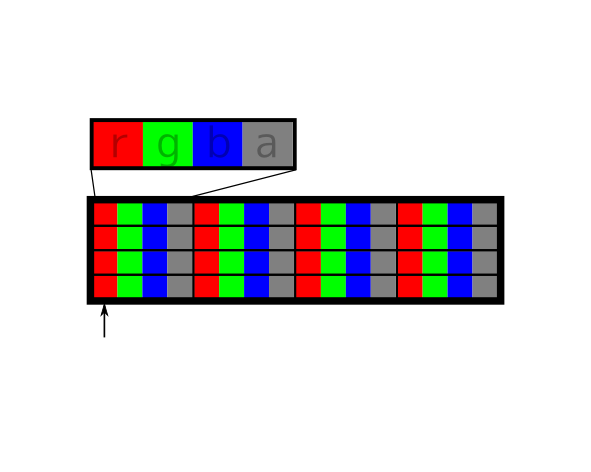
\includegraphics[width=0.5\textwidth]{images/tile-a} }
				\subfloat[Un tile aux canaux séparés]{ \label{fig:render-hsv} 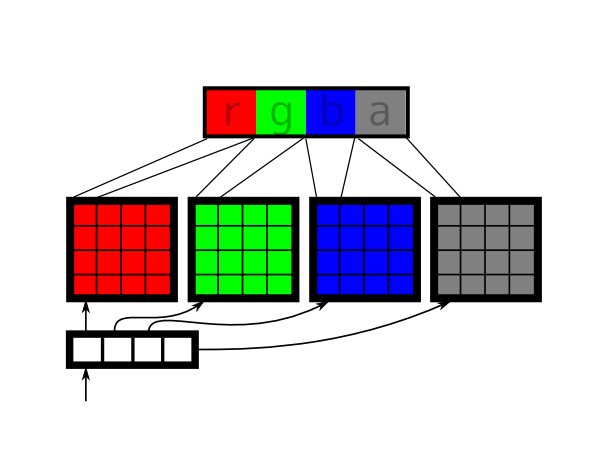
\includegraphics[width=0.5\textwidth]{images/tile-b} }
				\caption{Deux structures de tiles}
				\label{fig:tilestruct}
			\end{figure}
				\item[La répartition des pixels dans le tile] La manière commune de représenter un pixel au sein d'un bitmap est d'avoir
				toutes ses composantes placées dans des emplacement contigus. Une autre manière est de placer chaque composante dans un
				bitmap séparé. Un tile étant alors constitué de plusieurs bitmaps. L'intéret de cette technique est que les tiles de même
				quantisation ont la même taille en pixel, et les bitmaps les constituant la même taille en mémoire. Un autre intérèt est
				qu'il est maintenant beaucoup plus facile de programmer des opérations qui peuvent gérer un nombre quelconque de composantes
				par pixel.

				Cependant, cela implique que l'accès à un pixel nécessite autant d'accès mémoires que de composantes, ce qui ralentit 
				l'exécution du programme. 
			\end{description}

		\subsubsection{Comparaison des tiles}
			Le tableau TODO représente le résultat d'expériences qui résument les concepts précedemment exposés. Dans ce tableau, deux opérations
			sont testées : \emph{colorfill} consiste à remplir une image de $8192^2$ pixels \emph{RGBA} 8bits/composante d'une couleur unie. \emph{blend} consiste 
			en fusionner deux images de $8192^2$ pixels \emph{RGBA} 8 bits/composante par opacité. Ces deux opérations 
			sont utilisées très couramment pour la réalisation de peintures. 

			Ces opérations sont appliquées selon des schémas différents: \emph{colorfill\_full} remplit tous les tiles de l'image, alors que \emph{colorfill\_single}
			remplit un tile choisit au hasard autant de fois qu'il y a de tiles dans l'image. Le même nombre de pixels est donc traité dans les deux tests,
			mais le second devra accéder régulièrement à de nouvelles zones mémoire.

			Même chose pour les operations \emph{blend} : \emph{blend\_full} fusionne les tiles des deux images, \emph{blend\_single} fusionne deux tiles
			sélectionnés au hasard, \emph{blend\_intermediate} fusionne toute l'image sur un seul tile. Ce dernier test est fort représentatif de la
			manière dont les tiles sont utilisés dans Himalaya.

			Ensuite les tiles normales sont comparées aux tiles à canaux séparés. 
			

			\begin{table*}
				\label{tileperf}
				\tiny
				\begin{tabular*}{\textwidth}{@{\extracolsep{\fill}} | r | c || c | c | c | c | c | c | c | c | c |}
					\hline
					\multicolumn{2}{|r||}{Largeur des tiles}& 8	& 16	& 32	& 64	& 128	& 256	& 512	& 1024	& 2048	\\
					\hline 
					Test	& Tile &\multicolumn{9}{ c|}{Temps de calcul moyen sur 5 expériences (secondes)}\\
					\hline
					\emph{colorfill\_single} & Normal 	& 0.78	& 0.64 	& 0.58	& 0.57	& 0.49	& 0.28	& 0.28	& 0.28	& 0.31	\\
					\emph{colorfill\_full} & Normal 	& 1.14	& 0.7 	& 0.65	& 0.63	& 0.55	& 0.44	& 0.47	& 0.44	& 0.51	\\
					\emph{colorfill\_single}& Séparé 	& 1.30	& 1.06 	& 1.04	& 1.06	& 0.97	& 0.79	& 0.79	& 0.79	& 0.80	\\
					\emph{colorfill\_full} & Séparé 	& 2.14	& 1.39 	& 1.16	& 1.12	& 1.10	& 1.03	& 1.00	& 1.01 & 1.01	\\
					\hline\hline
					\emph{blend\_single} & Normal 		& -	& 3.12 	& 2.98	& 3.0	& 3.08	& 4.16	& 13.58	& 19.97	& 22.60	\\
					\emph{blend\_inter} & Normal 		& -	& 5.31 	& 5.20	& 4.96	& 5.12	& 4.85	& 13.49	& 20.46	& 20.64	\\
					\emph{blend\_full} & Normal 		& -	& 5.39 	& 5.19	& 5.17	& 5.0	& 5.42	& 13.15	& 20.44	& 21.12	\\
					\emph{blend\_single}& Séparé		& -	& 6.29 	& 5.64	& 5.39	& 6.61	& 6.50	& 18.67	& 27.48	& 28.92	\\
					\emph{blend\_inter}& Séparé		& -	& 6.55 	& 5.69	& 5.50	& 6.55	& 6.74	& 20.22	& 27.77	& 27.48	\\
					\emph{blend\_full} & Séparé	 	& -	& 6.68 	& 5.82	& 5.45	& 6.59	& 6.78	& 18.39	& 27.41 & 27.23	\\
					\hline
				\end{tabular*}
			\end{table*}
			\begin{figure}[h]
				\centering
				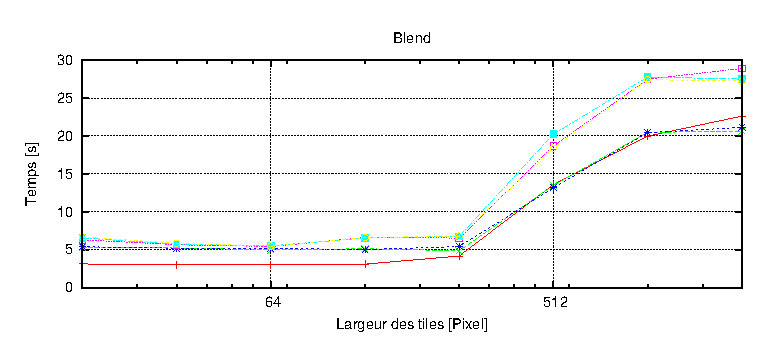
\includegraphics[width=\textwidth]{images/tilegraph.eps} 
				\label{fig:tilegraph}
			\end{figure}
		\subsubsection{Analyse des performances}
			On peut tirer plusieurs conclusion de ces expériences:
			\begin{itemize}
				\item Les tiles doivent être les plus grands possibles, pour diminuer le 
			nombre d'appels de fonctions, mais ne doivent pas être trop grands, sinon les performances sont très fortement dégradées. 
				\item Les tiles à canaux séparés sont jusque 2 fois plus lents que les tiles normaux.
				\item Le schémà d'accès aux tiles en mémoire a un impact non négligable mais plus marqué sur les tiles normaux.
				\item Le temps pour faire la fusion d'un même nombre de pixels peut différer de 970\% selon le type de tile, sa taille et la
				manière dont il est utilisé, puisque cette opération représente la grande majorité du temps de calcul du framework, ce choix
				est particulièrement important.
			\end{itemize}
			Enfin, il ne faut pas oublier que ces expériences ommettent deux facteurs importants: Le fait que la gestion des tiles dans le framework 
			est bien plus lourde, ce qui favorise les tiles plus grands, et le fait que les tiles plus petits permettent plus de précision dans 
			la localisation des opérations, ce qui permet de réduire le nombre de pixels accédés à chaque opération.

			Déterminer l'importance de ces deux facteurs requiert d'avoir des données d'utilisation du framework représentatives, par exemple
			avec des tests utilisateur. 
		\subsubsection{Structure finale}
			Le choix s'est porté sur des tiles normaux de taille fixe de $32\times32$ pixels, et ce quelque soit le modèle colorimétrique utilisé.

		\subsection{Les Frames}
			La Frame est la structure de donnée qui organise les tiles. Elle doit remplir plusieurs fonctions: stocker une image gigapixel,
			stocker les mipmaps de cette image, et servir de cache aux résultats des opérations, ainsi que les mipmaps de ceux-ci.

			L'intérèt des mipmaps est que pour un coût mémoire de seulement 33\% de l'image originale, ils permettent d'accéder à une sous région
			de l'image à une échelle quelconque en un temps ne dépendant que de la taille de cette sous-région, et non de la taille de l'image. 
			Cette propriété est indispensable pour pouvoir travailler sur des images giga-pixel.
			
			La Frame est une pyramide de tile creuses. Cette structure n'est pas nouvelle et est utilisée dans la pluspart des logiciels devant
			gérer des images gigapixel et leurs mipmaps. Les formats d'échange standard des photos satellites sont par exemple basés sur ces structures.
			
			L'intérèt d'avoir une pyramide creuse est de pouvoir stocker des tiles individuels, ce qui est indispensable pour pouvoir s'en servir
			comme d'une cache.

			Il existe plusieurs structures permettant l'organisation de tiles en pyramide creuses. La plus populaire est le quadtree, et c'est celle
			qui fut choisie pour l'implémentation des Frames.

			\subsubsection{Les quadtrees}
		\begin{lstlisting}[float,caption={Définition des hlFrameNodes},frame=tb,label=lsthlFrameNode]
typedef struct hl_frame_node{
	/* abscisse du tile */
	int tx;
	/* ordonnee du tile */
	int ty;
	/* tile  */
	hlTile *tile;
	/* Noeuds enfants */
	hlFrameNode *tl;
	hlFrameNode *tr;
	hlFrameNode *bl;
	hlFrameNode *br;
}hlFrameNode;
		\end{lstlisting}
				Les quadtrees sont composés de noeudsayant chacun une référence optionelle vers un tile, et de quatre références vers
				les noeuds enfants. 

				Chaque ensemble de noeuds de la même profondeur représente ainsi un bitmap à l'échelle deux fois plus petite que l'ensemble de
				noeuds à la profondeur suivante.

				Une définition de la structure des noeuds se trouve au listing~\ref{lsthlFrameNode}, page~\pageref{lsthlFrameNode}

			\subsubsection{Placer une image dans le Quad-Tree}
				Afin d'éviter d'avoir des Quad-Trees inutilement profond, les images sont stoquées au niveau le moins profond pouvant les contenir,
				soit $ceil( \log_2( max(size_x,size_y)/32))$, $size_x$,$size_y$ représentant la largeur et la hauteur de l'image en pixels.
				Cette profondeur est ensuite stoquée dans la Frame afin de pouvoir identifier le niveau correspondant à la résolution native.

			\subsubsection{Référencer les Tiles dans le Quad-Tree}
				Les tiles sont référencés par trois coordonnées $(t_x,t_y,t_z)$. $t_x,t_y$ représente les coordonnées spatiales du tile, $t_x$ valant
				zéro à l'extrémité gauche du bitmap, et étant positif à droite. $t_y$ vaut zéro à l'extrémité supérieure du bitmap et est positif vers le bas,
				et ce quelque soit l'échelle représentée.
				
				$t_z$ représente le niveau d'échelle. Il représente habituellement la profondeur du noeud à laquelle on trouve le tile. Nous avons
				choisi d'utiliser un système différent, $t_z$ vallant $0$ au niveau correspondant à la résolution native, et étant positif
				pour les échelles intérieures. L'intérèt de ce système est que la référence d'un tile est indépendante de sa profondeur réelle,
				qui peut changer lorsque l'on insère ou retire des tiles dans celui-ci.
				
				On peut s'intéresser à la valeur maximale de $t_z$ qui dépend de la taille de l'image stockée dans le quadTree.
				Comme nous voulons pouvoir indexer les pixels indépendemment, la largeur de l'image ne peut dépasser
				\emph{MAX\_INT}, Ce qui correspond à une valeur maximale de $t_z$ de $26$ sur les architectures 32bits, avec des tiles de 32 pixels
				de coté.
				
			\subsubsection{Les coordonnées négatives}
				Lorsque la Frame sert à stocker un bitmap chargé depuis le disque, les pixels le constituant, et donc les tiles, ont toujours des
				coordonnées $t_x,t_y$ positives. Cependant, il est pratique de pouvoir également stocker des pixels de coordonnées négatives, afin
				de disposer du plan complet pour pouvoir stocker le résultat de transformations géométriques. Pour ce faire, la Frame
				stoque un Quad-Tree par quadrant, et les tiles aux coordonnées négatives sont redirigées vers les Quad-Tree correspondant.

			\subsubsection{Le Tile de fond}
				Lorsque la frame est utilisée pour contenir un bitmap, celle-ci dispose d'un Tile de fond. Celui-ci n'est pas repris
				dans les Quad-Tree et est d'une couleur unie correspondant au 'fond' de l'image, habituellement une couleur transparente.
				Lorsque l'on tente d'accéder à une coordonnée qui ne correspond à aucun noeud des Quad-Trees, ce que l'on a atteint une zone
				correspondant au fond de l'image, et le tile de fond est renvoyé. Ceci permet de réduire l'espace mémoire consommé par les zones 
				vides des images.

			\subsubsection{Insertion, suppression et accès aux tiles}
				L'insertion, la suppression, et l'accès à un tile se fait en $O(n)$ ou $n$ est la profondeur à laquelle se trouve le tile dans 
				le Quad-Tree. Comme $n$ ne dépasse pas 26, le temps d'exécution de ces fonctions est borné, et on peut donc considérer que'elles
				ont une complexité de $O(1)$. 
				
				De plus l'insertion et la suppression augmentent ou diminuent automatiquement la taille des 
				quad-tree afin de s'assurer que la taille de l'arbre reste minimale. Ceci nécessite cependant de stocker à chaque noeud 
				sa coordonnée $t_x,t_y$, ce qui augmente leur taille de 40\%. TODO / evaluer l'espace pris.

			\subsubsection{Surchage mémoire}
				Les FrameNode ont un poids de $28$ Bytes, ce qui représente 2,66\% de la taille des tiles les plus petits(Alpha 8bit), 0.67\% de celle des plus
				communs(RGBA 8bit)  et 0.14\% de celle des plus grands(CMYKA 32bit). Dans le meilleur des cas, le stockage d'un tile ne 
				nécessite qu'un noeud, et 26 dans le pire des cas. On observe lors des tests utilisateurs qu'en moyenne le stockage d'un tile
				nécessite TODO noeuds, ce qui représente TODO pourcent.
			\subsubsection{Définition de l'hlFrame}
		\begin{lstlisting}[float,caption={Définition des hlFrames },frame=tb,label=lsthlFrame]
typedef struct hl_frame{
	/* largeur en pixel du bitmap */
	int sizex;
	/* hauteur en pixel du bitmap */
	int sizey;
	/* tile de fond */
	hlTile *bg;
	/* QuadTrees */
	hlFrameNode *tl;
	hlFrameNode *tr;
	hlFrameNode *bl;
	hlFrameNode *br;
}hlFrame;
		\end{lstlisting}
				On trouve 

		\subsection{L'hlImage}
		\begin{lstlisting}[float,caption={Définition des hlImages },frame=tb,label=lsthlImage]
typedef struct hl_image{
	/* Reference vers la derniere operation de la pile*/
	hlOperation *top;
	/* Reference vers la frame contenant le bitmap 
	 * a modifier */
	hlFrame *source;
}hlImage;
		\end{lstlisting}
		Si la frame représente une cache ou un bitmap, l'hlImage représente une image à proprement parler. L'hlImage est composée principalement
		de deux choses, une Frame représentant la source, c'est à dire une image de départ à modifier, et une liste, ou plutôt pile d'opérations
		qui modifient l'image.	
		Une défintion de la structure se trouve au Listing~\ref{lsthlImage}, page~\pageref{lsthlImage} 
		\subsubsection{La pile d'opérations}
			La pile d'opération est une liste simplement chainée d'opération. Chaque opération référence l'opération \emph{précédente}.
			L'\emph{hlImage} référence uniquement la \emph{dernière} opération. On peut se représenter ces opérations comme une pile,
			ou les opérations sont à appliquer au dessin de haut en bas, l'hlImage référençant le dessus de la pile. 
		\subsection{Les hlOperations}
		\begin{lstlisting}[float,caption={Définition des hlOperations },frame=tb,label=lsthlOp]
typedef struct hl_operation{
	/* Reference vers la classe de l'operation */
	hlOpClass  *class;	
	/* Reference vers l'operation precedente. */
	struct hl_operation *down;
	/* Frame qui sert de cache aux resultats de 
	 * l'operation */
	hlFrame *cache;			
	/* Reference vers l'image a laquelle appartient 
	 * l'operation */
	hlImage *image;			
	/* HL_MODIFABLE, HL_CACHING */
	int	 flags;			
	/* Un compteur de references */
	int	 refcount;		
	/* Les parametres de l'operation */
	void	*params;		
}hlOperation;
		\end{lstlisting}
		Les hlOperations sont les objets qui représentent toutes les opérations qui permettent de modifier une image. Une définition de la structure
		se trouve au Listing~\ref{lsthlOp}, page~\pageref{lsthlOp}. Certaines opérations particulières pouvant étendre cette structure avec des
		champs supplémentaires, qui seront détaillés dans les sections appropriées.

		Cela représente un minimum de 28Bytes\footnote{La structure telle qu'implémentée possède de nombreux champs supplémentaires à de fins de déboguage et fait
		92Bytes} par opération sur une architecture 32bits. Une hlOperation est donc suffisemment légère pour
		que l'on puisse en utiliser plusieurs millions sans problèmes de mémoire. 

		\subsubsection{La classe d'opération}
			\begin{lstlisting}[float,caption={Définition des classes d'opérations },frame=tb,label=lsthlOpClass]
typedef struct hl_op_class{
	/* HL_COLORFILTER, HL_FILTER, HL_DRAW, HL_BLEND */
	int category;
	/* Numero de l'operation*/
	int id;
	/* le nombre de parametres flottants */
	int float_param_count;
	/* le nombre de parametres entiers */
	int int_param_count;
	/* le nombre de parametres de couleur */
	int color_param_count;
	/* le nombre de parametres d'images */
	int image_param_count;
}hlOpClass;
			\end{lstlisting}
			La classe d'opération contient la description d'un type d'opération, et tout ce qui est commun à ces opérations, Il n'existe qu'une
			seule instance de chaque classe d'opération. La définition de ces classe est donnée au listint~\ref{lsthlOpClass}, page~\pageref{lsthlOpClass}.

			Les champs des classes d'opérations méritent d'être expliqués plus en détails	
			\begin{description}
				\item[\texttt{category}]. Les opérations sont divisées en plusieurs catégories, selon les propriétés et les paramètres
				nécessaires à l'application de l'opération. Ceci permettra d'appeler une méthode spécialisée pour chaque catégorie d'opération.
				Ces catégories correspondent également aux différentes catégories d'opération de dessin que nous avons vu au premier chapitre. 
				\begin{description}
					\item[\texttt{HL\_COLORFILTER}]: Les filtres colorimétriques. Ces filtres ne sont pas dépendants de la position du tile ou de son échelle, et s'appliquent
					sur toute l'image. 
					\item[\texttt{HL\_FILTER}]: Les filtres spatiaux. Ces filtres dépendent de l'échelle, de la position du tile, 
					et ne peuvent modifier un tile sans connaitre les données des tiles adjascents.
					\item[\texttt{HL\_DRAW}]: Le dessin de primitives. Ces opérations dépendent de l'échelle et de la position du tile, 
					mais ne s'appliquent que sur une sous-région de l'image.
					 Ces filtres dépendent de l'échelle et de la position du tile, et ne s'appliquent que sur
					une sous région de l'image.
					\item[\texttt{HL\_BLEND}]] Les opéartions de fusion. Ces opérations dépendent de la position du tile et de son échelle, 
					ainsi que d'une autre \emph{hlImage}
				\end{description}
				\item[\texttt{id}]Le numéro de l'opération, qui l'identifie dans sa catégorie. Par exemple, Le dessin de cercle 
				--- \texttt{HL\_DRAW\_CIRCLE} --- dans 
				la catégorie \texttt{HL\_DRAW}
				\item[\texttt{*\_param\_count}]: Le nombre de paramètres de chaque type. Les opérations sont limitées à quatre types de paramètres,
				les flottants, les entiers, les couleurs, et les images. Cette information est nécessaire pour pouvoir calculer la taille des 
				paramètres de la fonction. L'implémentation utilise un mécanisme similaire mais plus complexe permettant une introspection sur les
				paramètres.
			\end{description}
	\section{Algorithmes}
		\subsection{Dessin}
		Dans Himalaya, le dessin et la rasterisation sont deux opérations séparées et indépendantes. Le dessin consiste simplement à ajouter une opération.

			
		\subsection{Rasterisation}
	\section{États}
		\subsection{Sauvegarder l'état}
		\subsection{Charger un état}
		\subsection{Supprimer un état}
		\subsection{Modifier une opération}
	\section{Gestion de la cache}
	\section{Utilisation}
		\subsection{API publique}
		\subsection{Undo / Redo}
		\subsection{Modèle objet par calques}
		\subsection{Modèle objet nodal}
		\subsection{Traits de pinceau}

\chapter{Localité des operations (20 pages)}
	\section{Opérations vectorisées}
		\subsection{Impact sur l'API}
		\subsection{Évaluation des performances}
	\section{Bounding Boxes}
		\subsection{Algorithme Inline}
		\subsection{Algorithme Off-line}
		\subsection{Multi-Niveaux}
		\subsection{Impact sur l'API}
		\subsection{Évaluation des performances}

\chapter{Anti-aliasing (15 pages) }
	\section{Primitive de dessin}
	\section{Problèmes d'échelle}
		\subsection{Oversampling}
	\section{Problèmes de superposition}
	\section{Problèmes de bandes}
	\section{Problème de blending à faible opacité}
	\section{Problème de précision de positionement}
\chapter{Test utilisateurs (10 pages) }
	\section{Procédure}
	\section{Résultats}
	\section{Analyse}
\chapter{Comparaison d'Himalaya aux autres frameworks}
\chapter{Conclusion}
